\item \textbf{{[}ACJC/PRELIM/9569/2021/P1/Q7{]} }

A new social media platform is to be created. In years to come, it
is expected to be as popular globally as other trending social media
platforms.
\begin{enumerate}
\item Give two reasons why a NoSQL database is likely to be more suitable
than an SQL database for the social media platform. \hfill{}{[}2{]}
\end{enumerate}
A basic login page that controls access to user accounts is shown
below. The password field masks the user input with a dot (\textbullet )
replacing each of the characters supplied.
\noindent \begin{center}
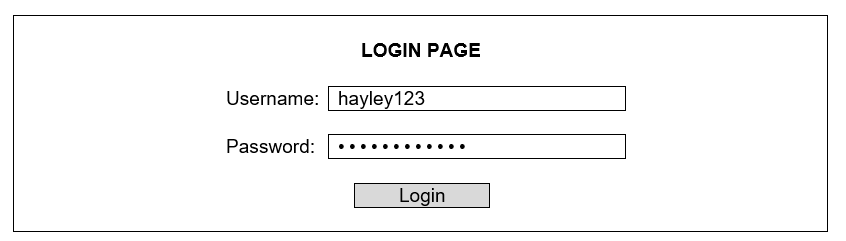
\includegraphics[scale=0.5]{C:/Users/Admin/Desktop/Github/question_bank/LyX/static/img/9569-ACJC-2021-P1-Q7}\quad{}
\par\end{center}
\begin{enumerate}
\item[(b)] When the login button is clicked, the program processes the username
and password supplied by the user.

It displays an error message if the username entered does not exist
in the database. If the password entered matches the registered password
for the username, login is granted. Otherwise, the program displays
an error message to indicate the user of the incorrect password entered.

The account will be locked if the user enters the correct username,
but enters the wrong password three times.
\begin{enumerate}
\item Create a decision table to show these conditions and actions. \hfill{}{[}4{]} 
\item Simplify your decision table by removing redundancies. \hfill{}{[}1{]} 
\end{enumerate}
\item[(c)] It is known that users tend to have different problems associated
with passwords.

Besides the error message to tell the user when an incorrect password
is entered, describe \textbf{two} examples based on usability principles
that can be applied to improve the functionality of the login page.
{[}2{]}
\item[(d)] Explain why the HTTP POST method should be used instead of the HTTP
GET method for the login request. \hfill{}{[}2{]}
\end{enumerate}